\begin{figure}[!htbp]
  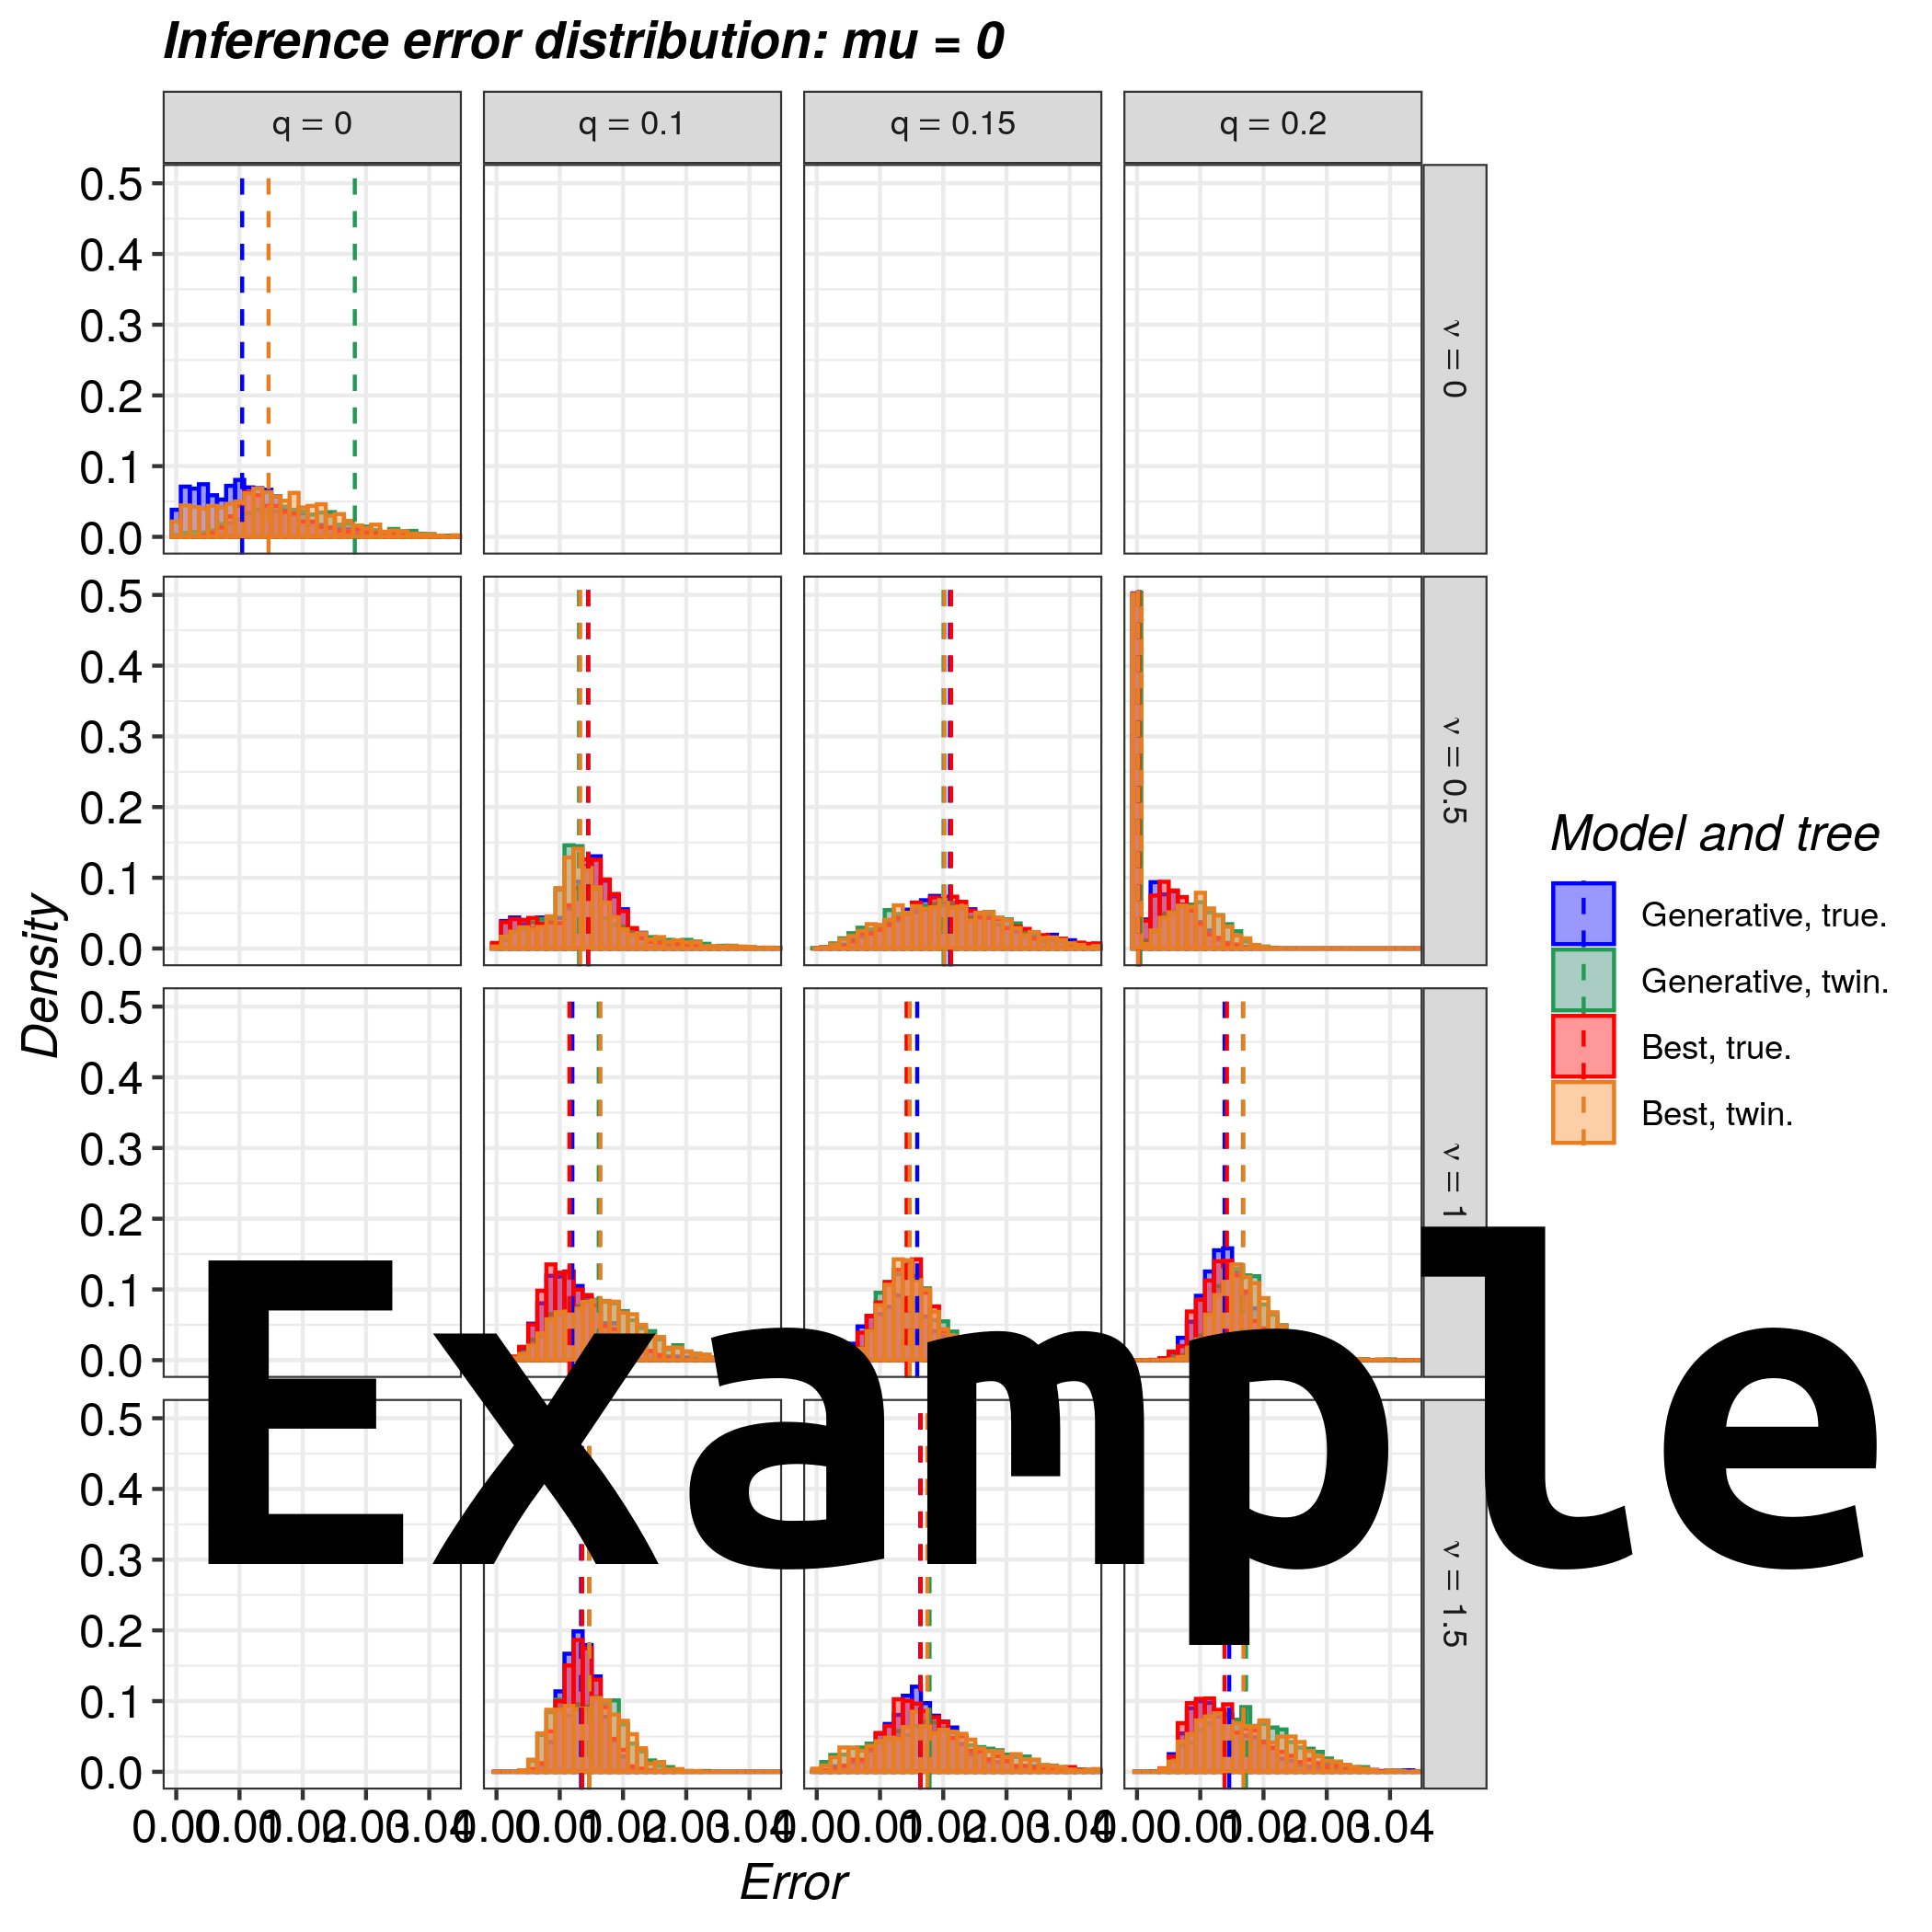
\includegraphics[width=\textwidth]{figure_1a.png}
  \caption{
    The error distribution for a extinction rate $\mu = 0.0$.
  }
  \label{fig:errors_yule}
\end{figure}

\begin{figure}[!htbp]
  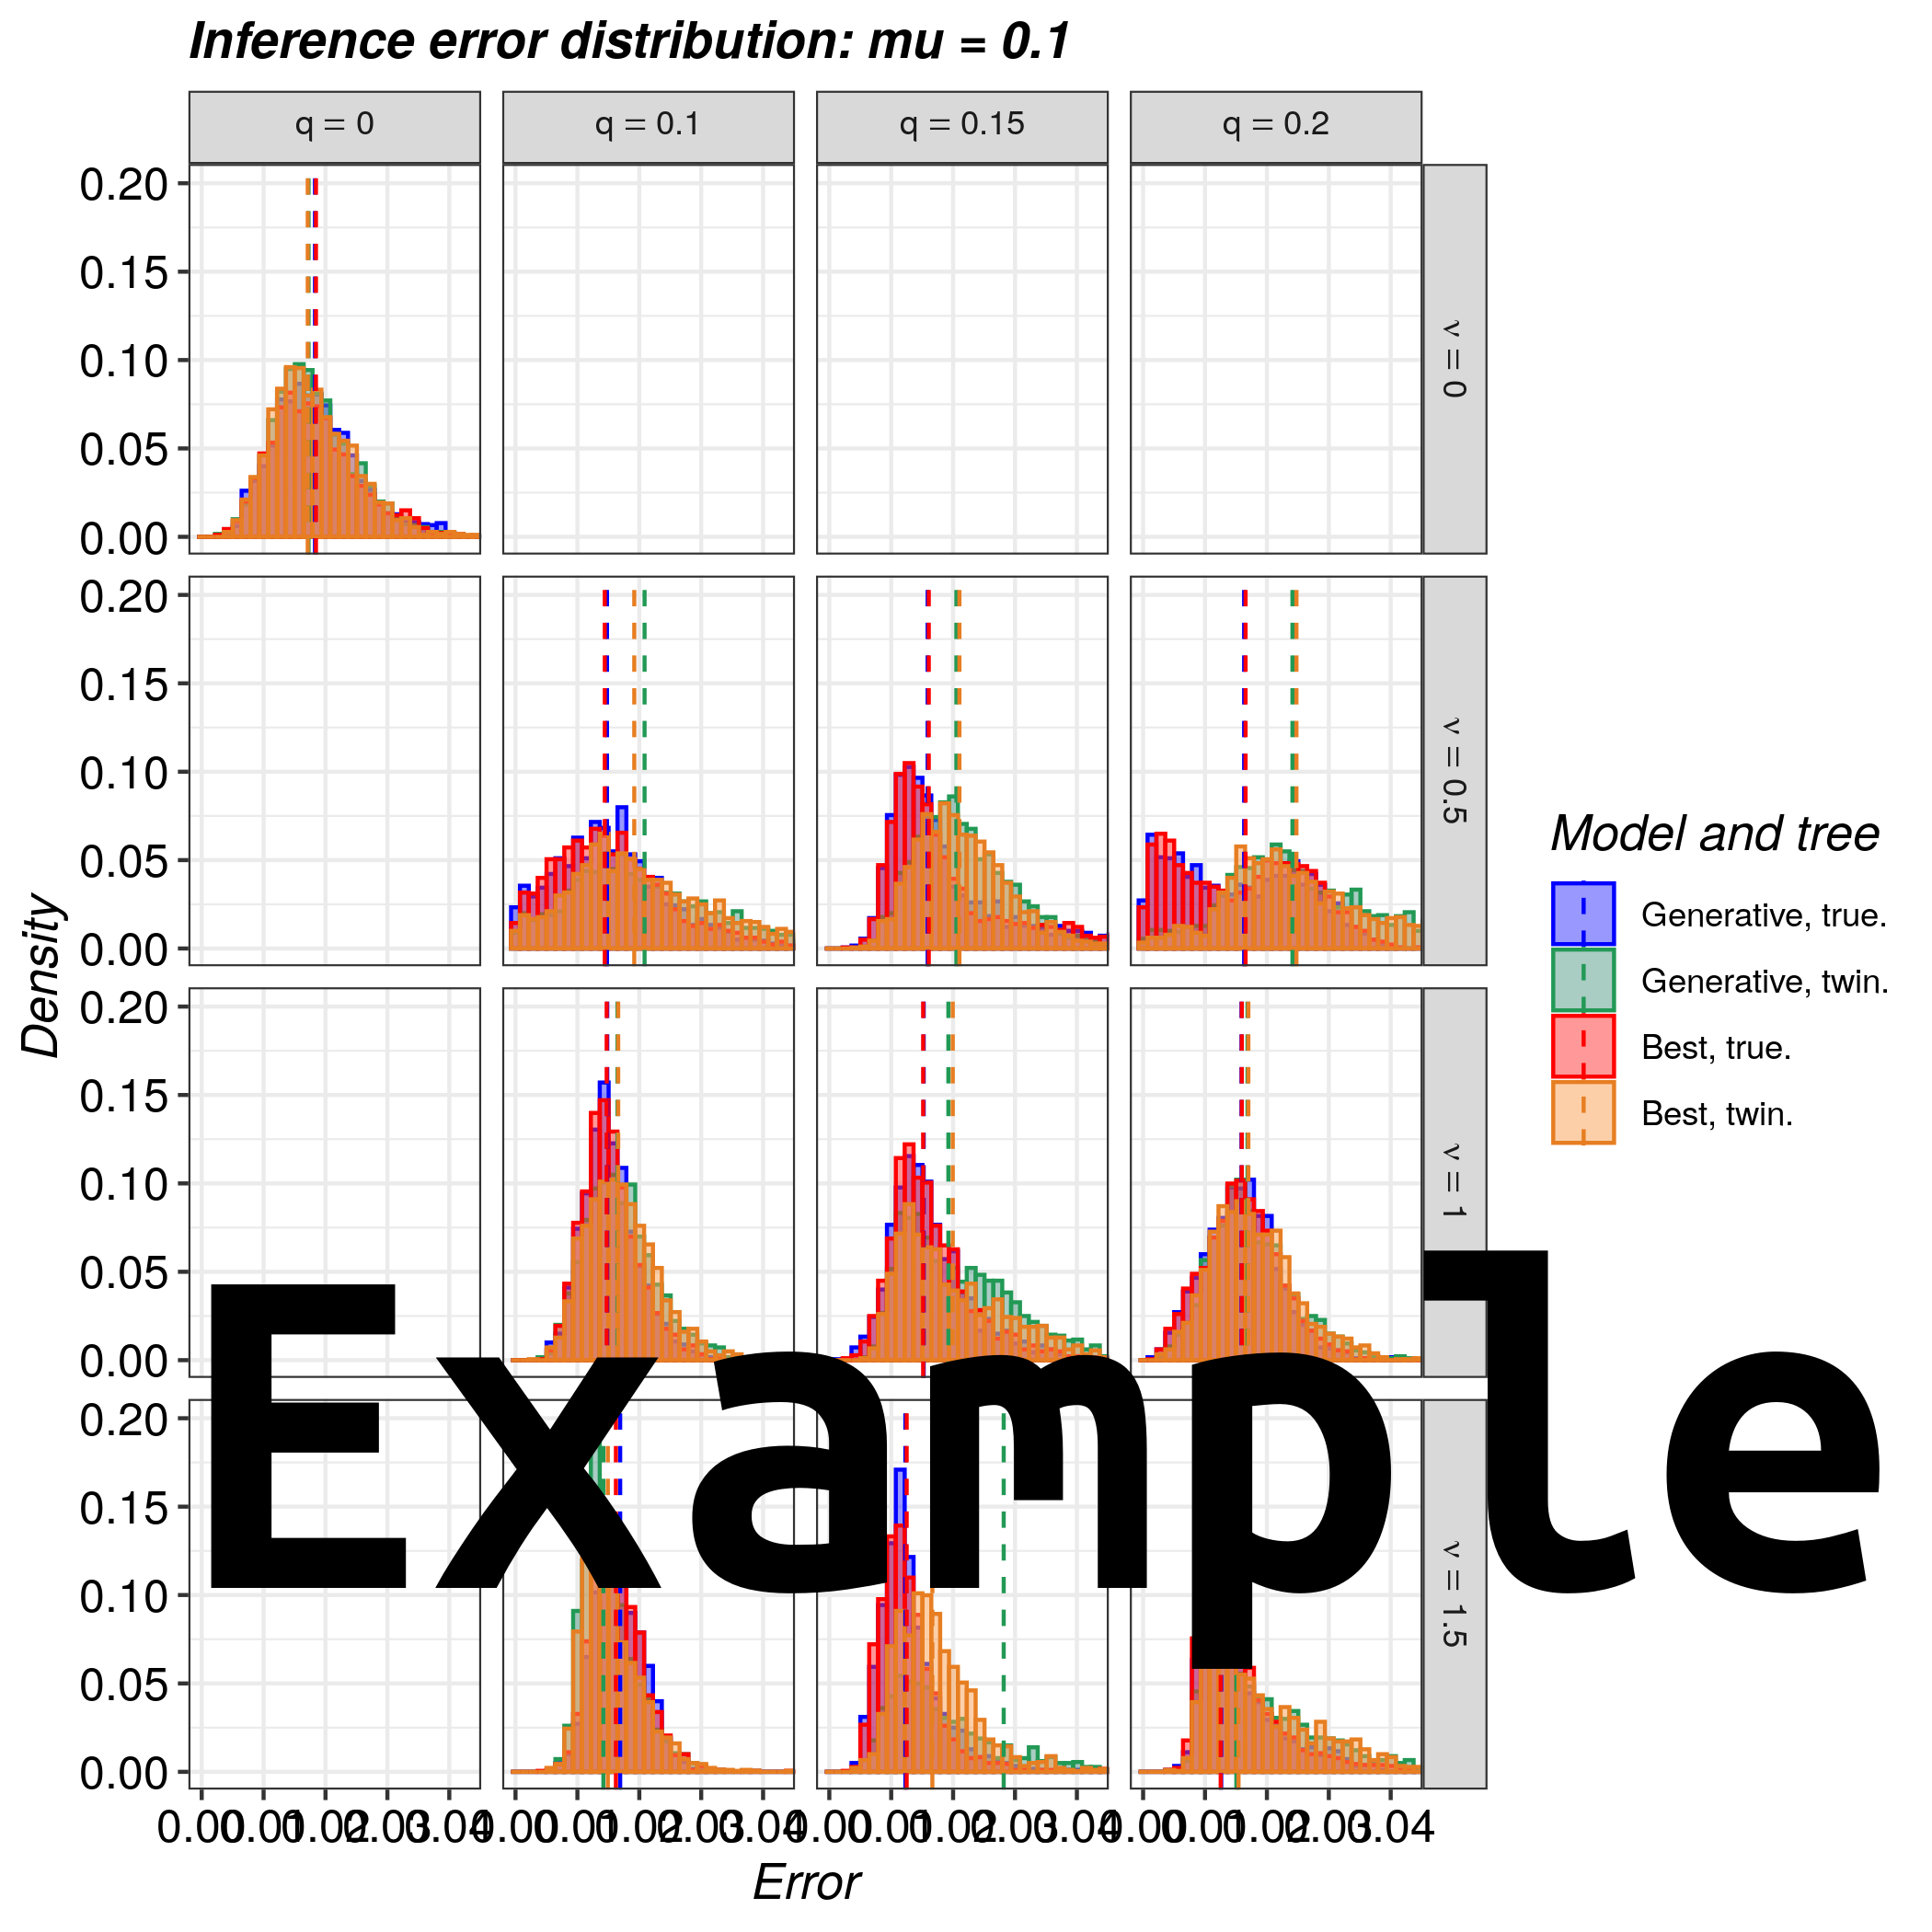
\includegraphics[width=\textwidth]{figure_1b.png}
  \caption{
    The error distribution for extinction rate $\mu = 0.15$.
  }
  \label{fig:errors_bd}
\end{figure}

\begin{figure}[!htbp]
  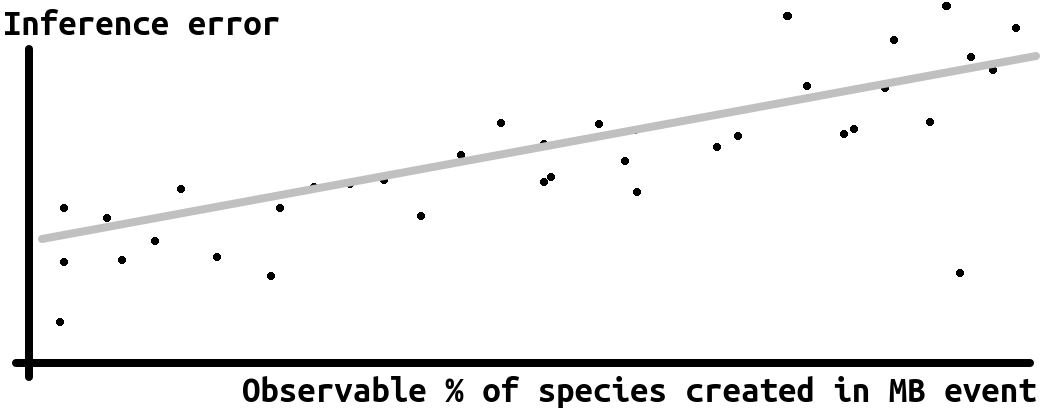
\includegraphics[width=\textwidth]{figure_2.png}
  \caption{
    The relation between percentage of observable MBness and
    the inference error. Each point corresponds to the error from
    one posterior tree.
  }
  \label{fig:mbness_and_error}
\end{figure}

\begin{figure}[!htbp]
  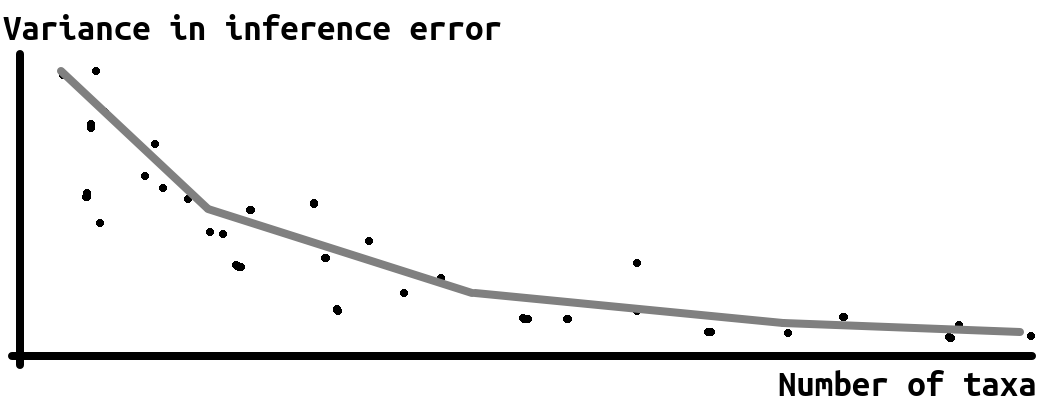
\includegraphics[width=\textwidth]{figure_3.png}
  \caption{
    The relation between the number of taxa and the
    variance of the inference error. 
    Each point corresponds to the variance of one posterior.
    \richel{move to supplementary materials?}
  }
  \label{fig:n_taxa_and_error_variance}
\end{figure}

\begin{figure}[!htbp]
  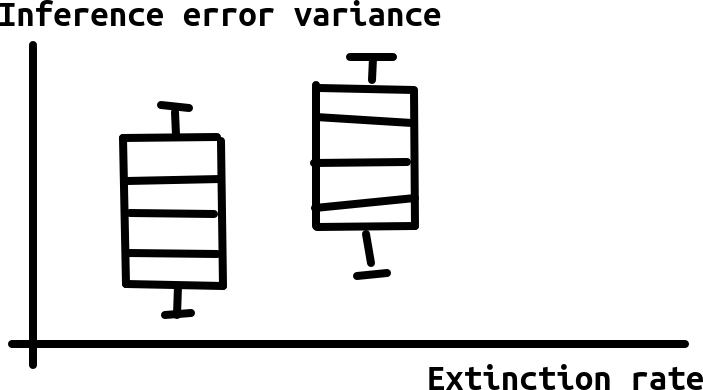
\includegraphics[width=\textwidth]{figure_4.png}
  \caption{
    The relation between the extinction rate and the
    variance of the inference error. 
    \richel{move to supplementary materials?}
  }
  \label{fig:ext_rate_and_error_variance}
\end{figure}

\begin{figure}[!htbp]
  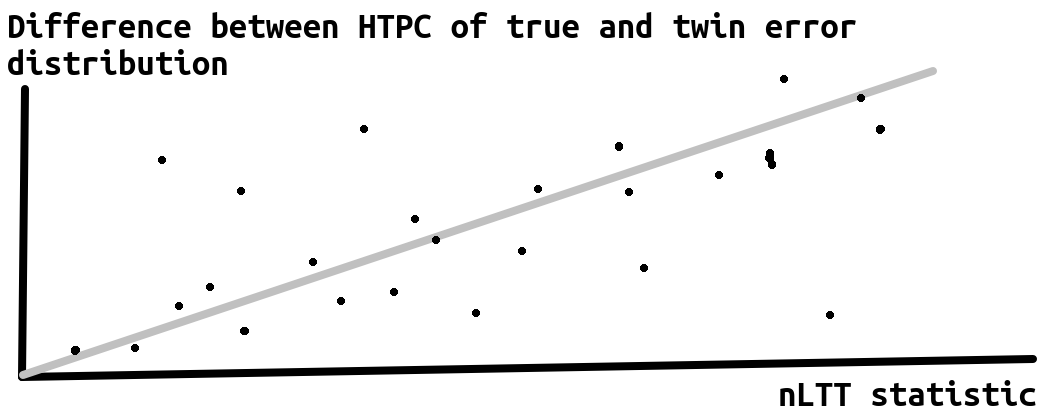
\includegraphics[width=\textwidth]{figure_5.png}
  \caption{
    The relation between the nLTT statistic and the difference
    between the HPD of the true and twin trees' errors. 
    Each point corresponds to the difference of 
    the HPD error between true and twin posterior.
    The grey line is the identity line.
  }
  \label{fig:nltt_and_error_difference}
\end{figure}

